% !TeX root = SA_Rockstroh_Main.tex
\chapter{Katalog von Modellen der Regelungstechnik}
\label{Ch:Ergebnisse}
% Ziel/Inhalt: Nur die Ergebnisse und keine großartigen Begründungen. Die sollen prinzipiell alle im vorherigen Kapitel stehen.
In diesem Kapitel werden die Ergebnisse der Studienarbeit vorgestellt. Angefangen wird mit der Struktur des Kataloges. Danach werden das Klassifikationssystem(s. \ref{Ch:Ergebnisse:Sec:KS}), die Modelldokumentation und die Modellimplementation(s. \ref{Ch:Ergebnisse:Sec:Dok+Implementierung}) als wichtige Elemente des Kataloges beschrieben. Eine Auflistung der aktuell vorhandenen Modelle(s. \ref{Ch:Ergebnisse:Sec:Modelle}) und eine Beschreibung des Ablaufes der Katalogerweiterung(s. \ref{Ch:Ergebnisse:Sec:Erweiterung}) schließen das Kapitel ab.
% Alternative Einführung: Like KS - Beschreibung was der Katalog ist.
% Einschub zur Terminologie: Etwas wird gemacht - ist schon umgesetzt. Etwas soll gemacht werden - noch nicht umgesetzt/praktiziert.
% ===========================================
% ------------- Katalogstruktur -------------
% ===========================================
\section{Katalogstruktur}
\label{Ch:Ergebnisse:Sec:Struktur}
Der Katalog besteht aus folgenden Elementen: Dem Klassifikationssystem, dem Python Package \textit{GeneralModel} und Modelleinträgen, die aus einer Metadaten-Datei, der Modelldokumentation, einer Parameter-Datei und, optional, aus der implementierten Modellklasse bestehen. Für jede Datei der Modelleinträge gibt es eine Vorlage. Die Beziehungen zwischen den Elementen sind in \ref{fig:katalogstruktur} dargestellt.

\begin{figure}
	\centering
	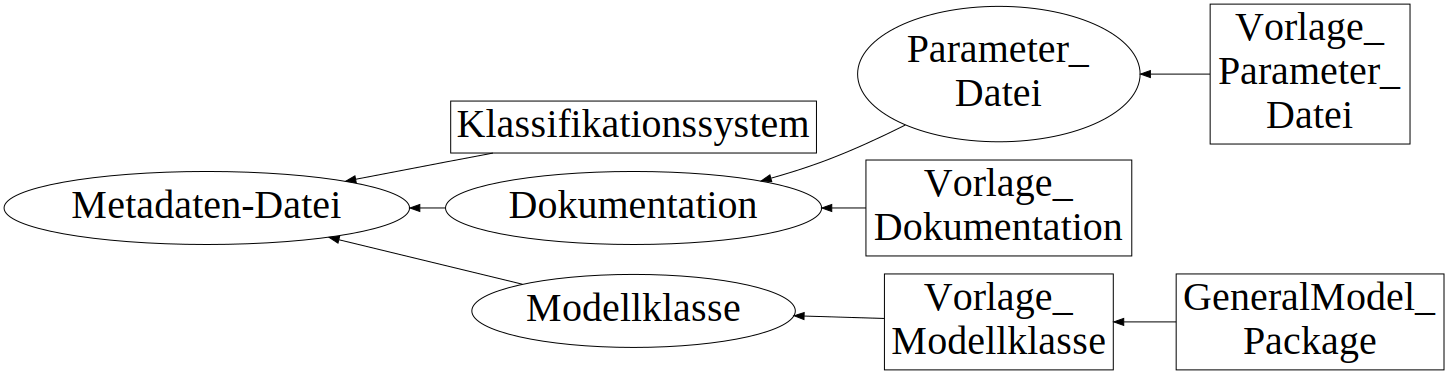
\includegraphics[width=1\linewidth]{Katalogstruktur}
	\caption[Katalogstruktur]{Elemente in Ellipsen existieren individuell für jedes Modell. Elemente in Rechtecken existieren genau ein Mal im Katalog.}
	\label{fig:katalogstruktur}
\end{figure}


Das \textit{Klassifikationssystem} ist eine Übersicht der Modelleigenschaften und deren Beziehungen untereinander. Die Einträge in dem Feld für die Modelleigenschaften in der Metadaten-Datei(tag\_list) sind nur Namen von Kategorieknoten aus dem KS. Es sorgt für eine einheitliche Namensgebung der Modelleigenschaften(s. Anforderung \ref{A.Modelleigenschaften}). 

Das Python Package \textit{GeneralModel} stellt die Python Klasse \textit{GeneralModel} zur Verfügung, von der alle Modellklassen der implementierten Modelle erben. Sie stellt ein Variablen- und Methodenset bereit, das alle Modellklassen gemeinsam haben.

Die \textit{Metadaten-Datei} ist eine Datei im YAML-Format, das Informationsfelder für Informationen zu dem zugehörigen Modell enthält. Das sind Felder für Informationen über das Modell (Modellname, Kurzbeschreibung, Modelleigenschaften, Dateinamen der Modellbilder), Felder für Informationen für eine Umsetzung des Kataloges als Datenbank(Key, Predecessor-Key, Implementation-Key) und weitere Informationen(Modellersteller, Erstellungsdatum, Liste der Bearbeiter, Externe Referenzen). Das Konzept und die Umsetzung der Metadaten-Datei stammt aus dem \textit{ACKRep}\footnote{ACKRep GitHub Repository: https://github.com/ackrep-org/ackrep\_data}.
% Noch schreiben welche Informationen im aktuellen Stand gegeben werden?

Die \textit{Modelldokumentation} ist die textuelle Notation des Modells. Sie wird in \LaTeX geschrieben. Nach jeder Bearbeitung wird die PDF-Datei aus der \LaTeX-Datei erzeugt. 

Die \textit{Parameter-Datei} ist eine Python-Datei. Diese enthält beispielhafte Parameterwerte für das Modell. Das Ausführen der Datei erzeugt eine Tabelle mit den beispielhaften Parameterwerten im \LaTeX-Format und schreibt die in eine \textit{Parameter.tex}-Datei, die im Ordner der Modelldokumentation abgelegt wird. Außerdem stellt Sie eine Methode für die implementierte Modellklasse bereit.

Die implementierte \textit{Modellklasse} ist eine Python-Datei, welche das Modell als Python-Klasse enthält. 

Die \textit{Vorlagen} für die Metadaten-Datei, die Parameter-Datei, die Modelldokumentation und -implementation sind Dateien, welche den Arbeitsaufwand für das Anlegen neuer Modelle verringern sollen. Die repetitiven Elemente für die entsprechenden Dateien sind in den Vorlagen schon vorhanden, so dass nur die Modellspezifischen Elemente neu geschrieben werden müssen. Die Verwendung der Vorlagen stellt eine einheitliche Struktur der Dateien sicher.



% =================================================
% ------------- Klassifikationssystem -------------
% =================================================
\section{Klassifikationssystem}
\label{Ch:Ergebnisse:Sec:KS}
Das \textit{Klassifikationssystem (KS)} stellt eine Wissensrepräsentation der  Es lehnt stark an die in \cite{KNHE20a} eingeführte OCSE an von der es sich insofern unterscheidet, das im KS nur der Teilbereich des Wissens der Regelungs- und Steuerungstheorie enthalten ist, der sich auf regelungstechnische Systeme und Modelle bezieht. Die im KS verwendeten Bezeichnungen sollen in den Metadaten-Dateien der Modelle bevorzugt verwendet werden. 

% =============================================================
% ------------- Aufbau des Klassifikationssystems -------------
% =============================================================
\subsection{Aufbau des Klassifikationssystems}
\label{Ch:Ergebniss:Sec:KS:SubSec:Aufbau}
Das KS ist ein gerichteter Graph der aus Knoten und Kanten besteht. Es gibt folgende Knotentypen: Kategorie-, Objekt-, Werte, und Wertetypknoten. 
Die Kanten zeigen Beziehungen zwischen den Knoten des KS auf, die durch die Kantenbeschriftungen spezifiziert werden. Es gibt folgende Kantenbeschriftungen: \glqq is a\grqq, \glqq Value\grqq, \glqq Type\grqq und \glqq Object\grqq. Die Kategorieknoten, ohne Ursprungsknoten und die Knoten der Hauptkategorien, und Objektknoten können als Modellattribute interpretiert werden. In der Metadaten-Datei dürfen nur diese Knoten des KS eingetragen werden.

Es gibt drei Attribute die kein Kantenursprung sind. Diese stellen die Hauptkategorien des KS dar. 
\\
\textbf{Mathematische Eigenschaften}: \\
Umfasst Eigenschaften die durch die mathematische Repräsentation des Modells gegeben sind. % ... die aus der math. Rep. direkt hervor gehen. --> Äquivalenzbegriff von Willems

\textbf{Systemeigenschaften}: \\ % Eigenschaften unabhängig von Darstellungsform eines äquivalenten Systems
Umfasst Eigenschaften die aus der mathematischen Repräsentation mit Methoden aus der Regelungstechnik abgeleitet werden.

\textbf{Verwendung}: \\
Umfasst Anwendungsfälle und -bereiche in denen die Modelle häufig genutzt werden.

% ===========================================================================
% ------------- Technische Umsetzung des Klassifikationssystems -------------
% ===========================================================================
\subsection{Technische Umsetzung des Klassifikationssystems}
\label{Ch:Ergebnisse:Sec:KS:SubSec:TechUmsetzung}

% =========================================================================
% ------------- Modelldokumentation und Modellimplementierung -------------
% =========================================================================
\section{Modelldokumentation und Modellimplementierung}
\label{Ch:Ergebnisse:Sec:Dok+Implementierung}

% ==============================================
% ------------- Vorhandene Modelle -------------
% ==============================================
\section{Vorhandene Modelle}
\label{Ch:Ergebnisse:Sec:Modelle}

% ==============================================
% ------------- Katalogerweiterung -------------
% ==============================================
\section{Katalogerweiterung}
\label{Ch:Ergebnisse:Sec:Erweiterung}



